\documentclass[a4paper,10pt]{article}
\usepackage[a4paper, total={180mm, 257mm}]{geometry}

\usepackage[colorlinks,linkcolor=blue,bookmarks,bookmarksopen,pdfauthor=krom]{hyperref}

\usepackage{fontspec}
\setmainfont[Path = fonts/, Extension = .ttf, BoldFont = ipagp]{ipamp}

\usepackage[compact]{titlesec}
\titlespacing{\section}{0em}{*0}{1.8em}
\titlespacing{\subsection}{0em}{*0}{2.3em}
\titlespacing{\subsubsection}{0em}{*0}{1.7em}
\titleformat{\section}{\normalfont\Huge}{\thesection}{0em}{}
\titleformat{\subsection}{\normalfont\Large}{\thesection}{0em}{}
\titleformat{\subsubsection}{\normalfont\normalsize}{\thesection}{0em}{}

\setlength\parindent{4em}
\setlength\parskip{0em}
\renewcommand{\baselinestretch}{1.24}

\usepackage{fancyhdr}
\pagestyle{fancy}
\fancyhf{}
\renewcommand\headrulewidth{0pt}

\usepackage{graphicx}
\graphicspath{{images/}}

\usepackage[usenames, dvipsnames]{color}
\definecolor{GTSgreen}{rgb}{0.35, 0.64, 0.18}

\begin{document}

\noindent\begin{picture}(0,0)
\put(186,-65){
\includegraphics[width=49mm]{GTSLogo}}
\put(186,-123){\color{GTSgreen}\Huge\textbf{\scalebox{2.85}[2.6]{GTS}}}
\put(55,-370){\Huge\scalebox{1.45}[1.45]{GTS Instruction Manual}}
\put(220,-397){\normalsize 2016 / 3 / 24 /}
\end{picture}

\newpage

\begin{center}
{\Huge{Contents}}
\end{center}

\vspace{4.5em}

\noindent\LARGE Installation Settings\\[0.5em]
\large 01 \ Preparing the Scanner \& Driver\\
02 \ TWAIN Driver Environment Settings (※ EPSON Scan Ver. 5.3.1.4)\\
03 \ Pre-execution Settings (※ Please set as necessary)\\[1.0em]
\LARGE Execution \& Termination\\[0.5em]
\large 04 \ Execution Method\\
05 \ Termination Method\\[1.0em]
\LARGE Pre-scan Settings\\[0.5em]
\large 06 \ Setting Resolution, Rotation \& Capture Range\\
07 \ Setting Image Type\\
08 \ Sequential Scan \& Save File Registration\\
09 \ Sequential Scan Confirmation\\
10 \ Sequential Scan Edit\\[1.0em]
\LARGE Scan Execution \& Storage\\[0.5em]
\large 11 \ Sequential Scan Execution (\& Save)\\[1.0em]
\LARGE State Saving \& Rescanning\\[0.5em]
\large 12 \ Save State to Resume Work\\
13 \ Resume Work, or Do Work such as Rescanning\\[1.0em]
\LARGE Trace (Full-Color Image Binary)\\[0.5em]
\large 14 \ Trace Preparation\\
15 \ Trace Adjustment\\
16 \ Trace Save Execution \\[1.0em]
\LARGE Full-Color Scan \& Trace\\[0.5em]
\large 17 \ Trace \& Save Simultaneously, While Scanning Full-Color Images\\
\\
Appendix A How To Change the Image Display

\fancyfoot[L]{\begin{picture}(0,0)
\put(0,0){
\includegraphics[width=25.8em, height=0.25em]{GTSFooter}}
\end{picture}
\vskip -0.3em \textbf{GTS}
}
\fancyfoot[R]{\vskip 0.1em \textbf{\thepage}}

\newpage

\renewcommand{\baselinestretch}{1.40}

\normalsize

\phantomsection
\section*{Installation Settings}
\addcontentsline{toc}{section}{Installation Settings}

\phantomsection
\subsection*{01 \ Preparing the Scanner \& Driver}
\addcontentsline{toc}{subsection}{01 Preparing the Scanner \& Driver}

\noindent Connect the TWAIN scanner to your computer and turn on the power.\\
(EPSON DS - 50000, EPSON Scan Ver. 5.3.1.4 has been tested, other drivers are unconfirmed)\\
Install the TWAIN driver corresponding to the connected scanner,\\
please confirm that it works.\\
The TWAIN driver does not mix with other scanner models,\\
it will be installed independently.\\

\phantomsection
\subsection*{02 \ TWAIN Driver Environment Settings (※ EPSON Scan Ver. 5.3.1.4)}
\addcontentsline{toc}{subsection}{02 TWAIN Driver Environment Settings (※ EPSON Scan Ver. 5.3.1.4)}

\noindent a \ Run “EPSON Scan", \& open the “EPSON Scan" window,\par
\noindent\hskip 1.0em Click the “Preferences..." button to open the “Preferences" window\\
\\
b \ Click the “Preview" tab,\par
\noindent\hskip 1.0em Uncheck “Photo/film auto rotation (O)"\\
\\
c \ Click the “Color" tab,\par
\noindent\hskip 1.0em Uncheck “Always execute automatic exposure"\par
\noindent\hskip 1.0em Set  “Display gamma" to “1.8" (other values may be used as necessary)\\
\\
d \ Click the “Documents" tab,\par
\noindent\hskip 1.0em Set "Boundary compensation amount" to zero\\
\\
e \ Click the “Others" tab,\par
\noindent\hskip 1.0em Uncheck “Compress transfer"\\

\phantomsection
\subsection*{03 \ Pre-execution Settings (※ Please set as necessary)}
\addcontentsline{toc}{subsection}{03 Pre-execution Settings (※ Please set as necessary)}

\phantomsection
\subsubsection*{○ “Level", “Load Config...", “Save As Config..." Initial folder}
\addcontentsline{toc}{subsubsection}{○ “Level", “Load Config...", “Save As Config..." Initial folder}

\noindent Write in the file “gts\_install\_setup.txt".\\
(Place this file in the folder where “gts.exe" exists)\\
For example, if you specify “C:¥User¥public",\\
browser\_directory\_path “C:¥User¥public"\\
will be set to the initial folder.

\newpage

\noindent If not specified, it becomes “C:¥".\\

\phantomsection
\subsubsection*{○ Shortcut key setting for sequential scan execution}
\addcontentsline{toc}{subsubsection}{○ Shortcut key setting for sequential scan execution}

\noindent Write in the file “gts\_install\_setup.txt".\\
(Place this file in the folder where “gts.exe" exists)\\
You can only specify Space, Enter, \& Esc.\\
For example,\\[-1.25em]

\setlength{\tabcolsep}{0em}
\renewcommand{\arraystretch}{1.0}
\noindent\begin{tabular}{p{17.0em}l}
short\_cut\_key\_start\_scan & Enter\\
short\_cut\_key\_rescan & Space\\
short\_cut\_key\_next\_scans & Enter\\
short\_cut\_key\_stop\_scan & Esc\\
\end{tabular}\\[-0.5em]

\noindent will set the shortcut keys.\\

\phantomsection
\subsubsection*{○ Preset settings of scan area}
\addcontentsline{toc}{subsubsection}{○ Preset settings of scan area}

\noindent Write in the file “\_gts-scan\_area.txt".\\
Place it in one of the following places. The top is higher priority.\\[-1.25em]

\setlength{\tabcolsep}{0em}
\renewcommand{\arraystretch}{1.0}
\noindent\hskip 4.0em \begin{tabular}{p{13.0em}l}
Each user's home & ※Environment Variable Path → “\%HOMEDRIVE\%\%HOMEPATH\%"\\
All user profiles & ※Environment Variable Path → “\%ALLUSERSPROFILE\%"\\
Share home & ※Environment Variable Path → “\%PUBLIC\%"\\
\multicolumn{2}{l}{Folder where “gts.exe" resides}\\
\end{tabular}\\[1.0em]

\noindent Specify the position \& size of the scan area\\
For example,\\[-1.25em]

\setlength{\tabcolsep}{0em}
\renewcommand{\arraystretch}{1.0}
\noindent\begin{tabular}{p{8.5em}p{8.5em}p{8.5em}p{8.5em}l}
A3 & 0 & 0 & 43.18 & 29.718\\
NTSC\_in\_A3 & 1.778 & 0 & 39.624 & 29.718\\
HD\_in\_A3 & 0 & 2.714625 & 43.18 & 24.28875\\
\end{tabular}\\[-0.5em]

\noindent will set the desired format.\\
\\
Specify the aspect ratio of the scan area (horizontal by longitudinal)\\
For example,\\[-1.25em]

\setlength{\tabcolsep}{0em}
\renewcommand{\arraystretch}{1.0}
\noindent\begin{tabular}{p{8.5em}p{8.5em}p{8.5em}l}
aspect\_ratio & HD & 16 & 9\\
aspect\_ratio & NTSC & 4 & 3\\
\end{tabular}\\[-0.5em]

\noindent will set the desired aspect ratio.\\

\phantomsection
\subsubsection*{○ Position \& size of the display}
\addcontentsline{toc}{subsubsection}{○ Position \& size of the display}

\noindent Write in the file “\_gts-desktop.txt".\\
This file is in the home folder of the logon account.\\
Automatically saves at the end of the application.

\newpage

\phantomsection
\section*{Execution \& Termination}
\addcontentsline{toc}{section}{Execution \& Termination}

\phantomsection
\subsection*{04 \ Execution Method}
\addcontentsline{toc}{subsection}{04 Execution Method}

\noindent “gts.exe"\\
Execute this file.

\noindent\begin{picture}(0,0)
\put(52,-237){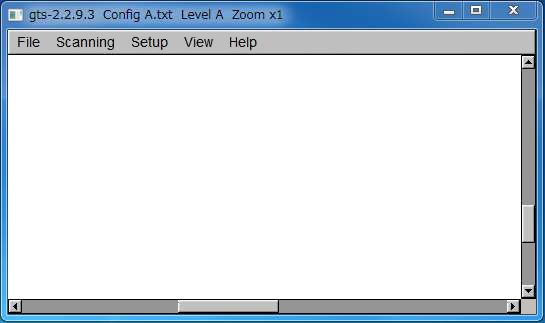
\includegraphics[width=143mm]{Config}}
\end{picture}\\[24.0em]

\noindent If you see a message saying, “Normal communication with the scanner can not be done..."\\
at this time\\
・ Check if the scanner cable is connected,\\
・ Check that the power switch is turned on,\\
・ Check that the driver has been properly installed,\\
please double check the above.\\

\phantomsection
\subsection*{05 \ Termination Method}
\addcontentsline{toc}{subsection}{05 Termination Method}

\noindent Select “Quit" from the “File" menu,\\
Click "Yes" on the confirmation dialog box displayed to exit.\\
\\
If you click "No", you can continue working without exiting.

\newpage

\phantomsection
\section*{Pre-scan Settings}
\addcontentsline{toc}{section}{Pre-scan Settings}

\phantomsection
\subsection*{06 \ Setting Resolution, Rotation \& Capture Range}
\addcontentsline{toc}{subsection}{06 Setting Resolution, Rotation \& Capture Range}

\noindent Select “Area and Rot 90..." on the “Setup" menu,\\
this will open the “Area and Rot 90" window.

\noindent\begin{picture}(0,0)
\put(171,-216){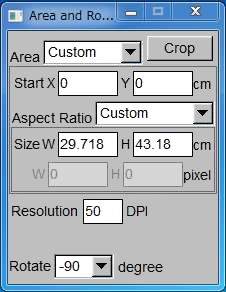
\includegraphics[width=59mm]{AreaAndRot90}}
\end{picture}\\[22.0em]

\noindent Information about the settings for “Resolution" → “Rotation" → “Capture Range", is shown below.\\

\phantomsection
\subsubsection*{○ Resolution}
\addcontentsline{toc}{subsubsection}{○ Resolution}

\noindent Click on the input part of “Resolution",\\
enter a numerical value from the keyboard.\\
The unit is Dot Per Inch.\\
\\
Please note that if you change the resolution after scanning with the “Crop" button,\\
you will need todo a “Crop" scan again.\\

\phantomsection
\subsubsection*{○ Rotation}
\addcontentsline{toc}{subsubsection}{○ Rotation}

\noindent It is specified in units of 90 degrees.\\
Please choose from the “Rotate" pull down options.\\

\phantomsection
\subsubsection*{○ Capture Range}
\addcontentsline{toc}{subsubsection}{○ Capture Range}

\noindent There are two setting methods, preset setting \& manual setting.

\newpage

\noindent Preset settings are specified in advance, inside a file,\\
select from the “Area" pull down options.\\
How to set presets\par
“03 Pre-execution Settings" → “○ Preset settings of scan area"\\
Please see the above section for details.\\
\\
Scan with manual settings \& specify the range while looking at the picture.\\
By pressing the “Crop" button, you can scan a picture through the entire range of the scanner,\\
it will be displayed on the screen. At the same time, a red frame \& small square are displayed.\\
A red frame indicates the range.\\
Drag the small square with the middle mouse button to change the range.\\
You can also enter numbers directly into the items “Start X", “Y", “Size W", “H".\\
How to change the overall display including images\par
“Appendix A How To Change the Image Display"\\
Please see the above section for details.\\
\\
If you want to set the aspect ratio to a specified ratio, use the “Aspect Ratio" preset.\\
How to set presets\par
“03 Pre-execution Settings" → “○ Preset settings of scan area"\\
Please see the above section for details.\\
When selecting from the “Aspect Ratio" preset, with the fixed width “W",\\
the height “H" value will change to the specified ratio.

\newpage

\phantomsection
\subsection*{07 \ Setting Image Type}
\addcontentsline{toc}{subsection}{07 Setting Image Type}

\noindent Select “Pixel Type and Bright..." from the “Setup" menu\\
this will open the “Pixel Type and Bright" window.

\noindent\begin{picture}(0,0)
\put(150,-152){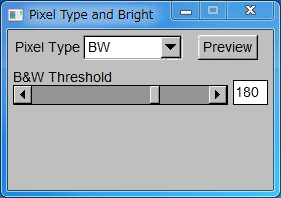
\includegraphics[width=73mm]{PixelTypeAndBright}}
\end{picture}\\[15.5em]

\phantomsection
\subsubsection*{○ Image Type “Pixel Type"}
\addcontentsline{toc}{subsubsection}{○ Image Type “Pixel Type"}

\noindent Select from the following three types.\\[-1.25em]

\setlength{\tabcolsep}{0em}
\renewcommand{\arraystretch}{1.0}
\begin{tabular}{p{8.5em}l}
BW & Black \& white monochrome binary image\\
Grayscale & Black \& white grayscale image\\
RGB & Full-color image\\
\end{tabular}\\[1.0em]

\phantomsection
\subsubsection*{○ Capture Adjustment}
\addcontentsline{toc}{subsubsection}{○ Capture Adjustment}

\noindent In the case of “BW", the binary conversion is made directly to black \& white during scanning.\\
Therefore, we decide the threshold (boundary) value of black \& white.\\
Change the “B\&W Threshold" with a value between 0 and 255,\\
Adjust the value while checking the image by repeating the scan,\\
and using the “Preview" button.\\
\\
“Grayscale", “RGB": In the case of “Brightness", “Contrast", “Gamma"\\
Although there are parameters, for basic use,\\
it is recommended to use all default values for these settings.

\newpage

\phantomsection
\subsection*{08 \ Sequential Scan \& Save File Registration}
\addcontentsline{toc}{subsection}{08 Sequential Scan \& Save File Registration}

\noindent Select “Level..." from the “File" menu\\
this will open the “Browse Level" window.

\noindent\begin{picture}(0,0)
\put(134,-351){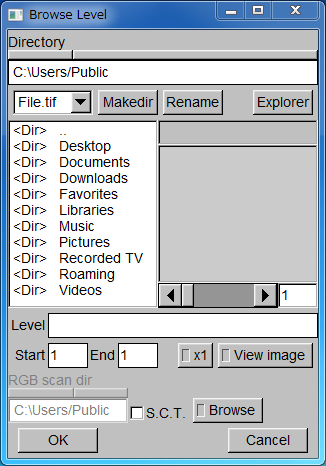
\includegraphics[width=85mm]{BrowseLevel}}
\end{picture}\\[34.0em]

\phantomsection
\subsubsection*{○ Set the storage location, name, start number \& end number of the sequential images}
\addcontentsline{toc}{subsubsection}{○ Set the storage location, name, start number \& end number of the sequential images}

\noindent using the following items,\\[-1.25em]

\setlength{\tabcolsep}{0em}
\renewcommand{\arraystretch}{1.0}
\begin{tabular}{p{8.5em}l}
“Directory" & Storage location\\
“Level" & (The beginning of the file) Name\\
“Start" & Start (frame) number\\
“End" & End (frame) number\\
\end{tabular}\\[-0.5em]

\noindent and click the “OK" button, to set the values.\\
\\
To change the “Storage location",\\
Click the desired folder from the list displayed on the left to move it.\\

\phantomsection
\subsubsection*{○ Creating a new folder}
\addcontentsline{toc}{subsubsection}{○ Creating a new folder}

\noindent Press the “Makedir" button, enter the folder name into the “New directory name" input part,\\
using the keyboard, and click the “OK" button.

\newpage

\noindent\vspace{0.5em}

\phantomsection
\subsubsection*{○ Renaming folders}
\addcontentsline{toc}{subsubsection}{○ Renaming folders}

\noindent While holding down the “Ctrl" key, click the folder to select it.\\
Then press the “Rename" button, using the “Rename Directory" input part,\\
change the folder name and click the “OK" button.\\

\phantomsection
\subsubsection*{○ When you want to perform other folder or file operations}
\addcontentsline{toc}{subsubsection}{○ When you want to perform other folder or file operations}

\noindent Please click the “Explorer" button which will open Windows Explorer.\\

\phantomsection
\subsubsection*{○ Save file format \& extension}
\addcontentsline{toc}{subsubsection}{○ Save file format \& extension}

\noindent The format of the image file which will be saved is TIFF.\\
Each file is automatically appended with the extension “tif".\\

\phantomsection
\subsubsection*{○ File name format}
\addcontentsline{toc}{subsubsection}{○ File name format}

\noindent For example,\\[-1.25em]

\setlength{\tabcolsep}{0em}
\renewcommand{\arraystretch}{1.0}
\begin{tabular}{p{8.5em}l}
“Level" & A\\
“Start" & 1\\
“End" & 2\\
\end{tabular}\\[-0.5em]

\noindent then,\par
“A.0001.tif”\par
“A.0002.tif”\\
will be the saved file names.\\

\phantomsection
\subsubsection*{○ Intermediate file name for full-color images}
\addcontentsline{toc}{subsubsection}{○ Intermediate file name for full-color images}

\noindent However, when “RGB" is selected for "Pixel Type",\par
“A.0001.tif"\\
"\_full" is automatically added to the name,\par
“A\_full.0001.tif"\\
will be the saved file name.

\newpage

\phantomsection
\subsection*{09 \ Sequential Scan Confirmation}
\addcontentsline{toc}{subsection}{09 Sequential Scan Confirmation}

\noindent Select “File Number..." on the “Setup" menu\\
this will open the “Number" window.

\noindent\begin{picture}(0,0)
\put(206,-283){
\includegraphics[width=34mm]{FileNumber}}
\end{picture}\\[28.0em]

\noindent Displays the sequential number of the start and end frames set by “Level",\\
and makes sure it is in selected state.\\[2.0em]

\phantomsection
\subsection*{10 \ Sequential Scan Edit}
\addcontentsline{toc}{subsection}{10 Sequential Scan Edit}

\noindent To delete frame numbers,\\
in the “Number" window, select only the frames you wish to delete,\\
if you select “Delete" from the “Edit" menu,\\
it will delete all the selected frames.\\
\\
To add a frame number,\\
click on the input entry directly under the menu in the “Number" window,\\
enter the new frame number using the keyboard and then press the Enter key to add it.\\
\\
When partially scanning a sequential number,\\
only the frame number is selected.

\newpage

\phantomsection
\section*{Scan Execution \& Storage}
\addcontentsline{toc}{section}{Scan Execution \& Storage}

\phantomsection
\subsection*{11 \ Sequential Scan Execution (\& Save)}
\addcontentsline{toc}{subsection}{11 Sequential Scan Execution (\& Save)}

\noindent Scanning will start as soon as you select “Scan" in the “Scanning" menu.

\noindent\begin{picture}(0,0)
\put(189,-74){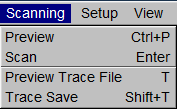
\includegraphics[width=46mm]{Scanning}}
\end{picture}\\[7.5em]

\noindent From the top, select the number selected in the “Number" window,\\
After scanning \& saving, an “S" mark will be added.\\
\\
When the first image is completed, the “Next" window will be displayed.

\noindent\begin{picture}(0,0)
\put(45,-100){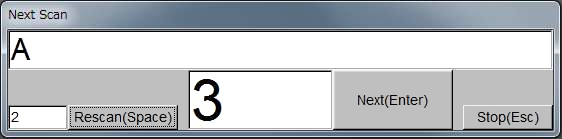
\includegraphics[width=148mm]{NextScan}}
\end{picture}\\[10.0em]

\noindent The following operations are performed with each button.\\[-1.25em]

\setlength{\tabcolsep}{0em}
\renewcommand{\arraystretch}{1.0}
\begin{tabular}{p{8.5em}l}
“Rescan" & → Rescan the current number\\
“Next" & → Scan the next number\\
“Stop" & → Cancel continuous scan\\
\end{tabular}\\[1.0em]

\noindent After scanning the last number, the “Next" window will not be displayed.

\newpage

\phantomsection
\section*{State Saving \& Rescanning}
\addcontentsline{toc}{section}{State Saving \& Rescanning}

\phantomsection
\subsection*{12 \ Save State to Resume Work}
\addcontentsline{toc}{subsection}{12 Save State to Resume Work}

\noindent Select “Save As Config..." on the “File" menu\\
this will open the “Save As Config" window.

\noindent\begin{picture}(0,0)
\put(145,-271){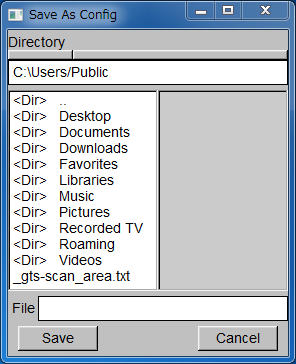
\includegraphics[width=78mm]{SaveAsConfig}}
\end{picture}\\[27.5em]

\noindent Navigate to the same place as “Level", give the same name and save with the “Save" button.\\
\\
“.txt" is appended automatically as an extension.\\
Even if you enter “.txt" at the end of the name, it will not be doubled.

\newpage

\phantomsection
\subsection*{13 \ Resume Work, or Do Work such as Rescanning}
\addcontentsline{toc}{subsection}{13 Resume Work, or Do Work such as Rescanning}

\noindent Select “Load Config..." on the “File" menu\\
this will open the “Load Config" window.

\noindent\begin{picture}(0,0)
\put(130,-278){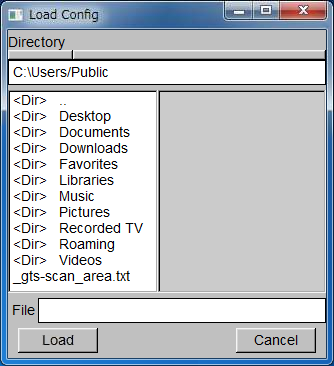
\includegraphics[width=88mm]{LoadConfig}}
\end{picture}\\[28.0em]

\noindent Select the saved file and click the “Load" button.\\
This will reproduce the work state.

\newpage

\phantomsection
\section*{Trace (Full-Color Image Binary)}
\addcontentsline{toc}{section}{Trace (Full-Color Image Binary)}

\phantomsection
\subsection*{14 \ Trace Preparation}
\addcontentsline{toc}{subsection}{14 Trace Preparation}

\noindent First, scan the full-color image.\\
\\
Select “Level..." from the “File" menu\\
this will open the “Browse Level" window.\\
\\
Specify the RGB image file using the following procedure.\par
\noindent\hskip 1.0em 1 Set the pull-down selection item at the bottom right of the “Directory" item of “Browse Level"\par
\noindent\hskip 2.0em to “Level.tif".\par
\noindent\hskip 1.0em 2 Move to the place where the scanned image is located and set the path to “Directory"\par
\noindent\hskip 1.0em 3 Click the image file name,\par
\noindent\hskip 2.0em and confirm the display of “Level", “Start", “End"\par
\noindent\hskip 1.0em 4 Click the “OK" button to close it\par
\noindent\hskip 1.0em 5 Confirm that the number and “S" are displayed in the “Number" window\\
\\
Display the image on the screen\\
If you select “Preview Trace File" on the “Scanning" menu\\
the first image of the selected number is displayed.\\
Incidentally,\\
when the Zoom value of the image is smaller than 1/2, the binary image will not be redisplayed\\
\\
How to change the display of the entire image\par
“Appendix A How To Change the Image Display"\\
Please see the above section for details.\\
\\
To display only images before binarization,\\
click “main\_to\_lr\_to\_sub" in the “Color Trace Window" of the “View" menu.\\
Click the same item again to undo.\\
\\
To display it separately from the top and bottom instead of right and left,\\
click “lr\_to\_ud" in the “Color Trace Window" of the “View" menu.\\
Click the same item again to undo.\\

\newpage

\phantomsection
\subsection*{15 \ Trace Adjustment}
\addcontentsline{toc}{subsection}{15 Trace Adjustment}

\noindent Select “Color Trace Enhancement..." from the “File" menu\\
this will open the “Color Trace Enhancement" window.

\noindent\begin{picture}(0,0)
\put(140,-645){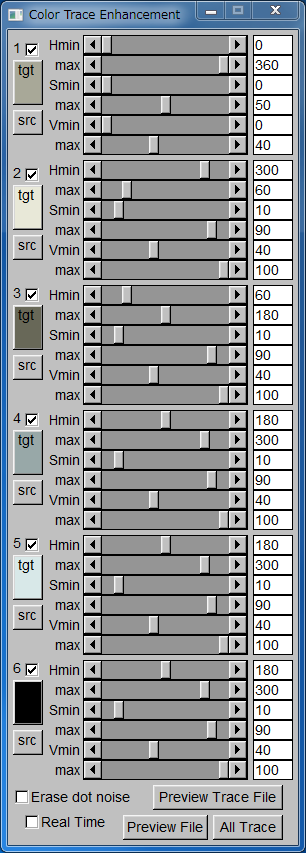
\includegraphics[width=81mm]{ColorTraceEnhancement}}
\end{picture}\\[28.0em]

\newpage

\noindent Information of how you can adjust while looking at the image, is shown below.\\
At this time, Zoom needs to be set to 1/2 or more,\\
please check the “Real Time" box.\\
\\
You can specify up to six colors from 1 to 6 to binarize.\\
\\
First, they will show initial values\par
if you inspect all the numbers on the right\par
all the items of Hmin, max, Smin, max, Vmin, max will be set to zero\\
(all from 1 to 6).\\
\\
Break the image up into the smallest amount of colors that you want to scan.\\
For example,\\[-1.25em]

\setlength{\tabcolsep}{0em}
\renewcommand{\arraystretch}{1.0}
\begin{tabular}{p{12.5em}l}
Highlight Color & Red Pencil\\
Black Line & Pencil\\
Shade Line & Blue Pencil\\
\end{tabular}\\[1.0em]

\noindent When binarizing these three colors\\
if you want to binarize in order of highlights and then the pencil lines,\\
use Red Pencil on 1, Pencil on 2, \& Blue Pencil on 3.\\
\\
Set the colors of the desired binarized result.\\
Click the “tgt" button to display the “Edit Color" window,

\noindent\begin{picture}(0,0)
\put(87,-107){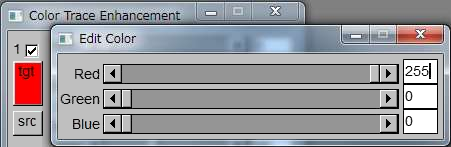
\includegraphics[width=118mm]{EditColor}}
\end{picture}\\[9.5em]

\noindent specify the color with the slide bars.\\
\\
Specify the color range to pick up as binarization.\par
Red Pencil adjustment example\\[-1.25em]

\setlength{\tabcolsep}{0em}
\renewcommand{\arraystretch}{1.0}
\hspace{4.0em}\begin{tabular}{rl}
Hmin \hspace{1.0em}  & 330\\
max \hspace{1.0em} & 30\\
Smin \hspace{1.0em} & Smaller values makes the line thicker, larger values makes the line thinner\\
max \hspace{1.0em} & 100\\
Vmin \hspace{1.0em} & 0\\
max \hspace{1.0em} & 100\\
\end{tabular}\\[-0.5em]

Black Line adjustment example\\[-1.25em]

\setlength{\tabcolsep}{0em}
\renewcommand{\arraystretch}{1.0}
\hspace{4.0em}\begin{tabular}{rl}
Hmin \hspace{1.0em} & 0\\
max \hspace{1.0em} & 360\\
\end{tabular}

\newpage

\setlength{\tabcolsep}{0em}
\renewcommand{\arraystretch}{1.0}
\hspace{4.0em}\begin{tabular}{rl}
Smin \hspace{1.0em} & 0\\
max \hspace{1.0em} & 100\\
Vmin \hspace{1.0em} & 0\\
max \hspace{1.0em} & Larger values makes the line thicker, smaller values makes the line thinner\\
\end{tabular}\\[-0.5em]

Blue Pencil adjustment example\\[-1.25em]

\setlength{\tabcolsep}{0em}
\renewcommand{\arraystretch}{1.0}
\hspace{4.0em}\begin{tabular}{rl}
Hmin \hspace{1.0em} & 210\\
max \hspace{1.0em} & 270\\
Smin \hspace{1.0em} & Smaller values makes the line thicker, larger values makes the line thinner\\
max \hspace{1.0em} & 100\\
Vmin \hspace{1.0em} & 0\\
max \hspace{1.0em} & 100\\
\end{tabular}\\[-0.5em]

\noindent Button Explanation\par
Erase dot noise\par
\hspace{4.0em} If checked, 1 dot noise will be erased.\par
\hspace{4.0em} Automatically block dust points and 1 dot holes on the line.\par
Real Time\par
\hspace{4.0em} If checked, shows real time changes of numerical values,\par
\hspace{4.0em} or each time you scroll, the binary image will be redisplayed.\par
\hspace{4.0em} This does not work when the Zoom is 1/4 or less.\par
\hspace{4.0em} Please set the Zoom to 1/2 or more.\par
Preview Trace File\par
\hspace{4.0em} Redisplays the image selected in the “Number" window\par
\hspace{4.0em} and the binarized image.\par
Preview File\par
\hspace{4.0em} This will redisplay only the image selected in the “Number" window.\par
All Trace\par
\hspace{4.0em} The binarized image is redisplayed from the current image.\\

\phantomsection
\subsection*{16 \ Trace Save Execution}
\addcontentsline{toc}{subsection}{16 Trace Save Execution}

\noindent If you select “Trace Save" from the "Scanning" menu\\
it will read the file and save it while binarizing it.\\
\\
Cancellation can not be canceled.\\
\\
It will be saved it in the same place as the input image.\\
\\
If the input image is “A\_full.0001.tif", it will be saved with the filename “A.0001.tif".

\newpage

\phantomsection
\section*{Full-Color Scan \& Trace}
\addcontentsline{toc}{section}{Full-Color Scan \& Trace}

\phantomsection
\subsection*{17 \ Trace \& Save Simultaneously,\\[0.75em]
\phantom{}\hspace{2.0em} While Scanning Full-Color Images}
\addcontentsline{toc}{subsection}{17 Trace \& Save Simultaneously, While Scanning Full-Color Images}

\noindent When scanning is performed with “S.C.T." (Save Color Trace level) checked in the “Browse Level" window,\\
binarized images are saved at the same time.\\
For example,\\
full-color image is “A\_full.0001.tif"\\
binary image is \hskip 1.2em “A.0001.tif"\\
will both be saved in the same place with the names above.\\
\\
You can specify a location to store full-color images separately.\\
First, on the right of “RGB scan dir" in the “Browse Level" window,\\
click the “Browse" button to turn it ON.\\
Next, navigate to the place to save, to change the path of “RGB scan dir".\\
Then, click the “OK" button to close it and execute the scan,\\
only the full-color images will be saved in this other designated location.

\newpage

\phantomsection
\subsection*{Appendix A How To Change the Image Display}
\addcontentsline{toc}{subsection}{Appendix A How To Change the Image Display}

\setlength{\tabcolsep}{0em}
\renewcommand{\arraystretch}{1.0}
\noindent\begin{tabular}{p{8.5em}l}
Translation & Drag with the middle mouse button (you are outside the frame if there is a small rectangle)\\
Expand &  Left mouse button or ‘z' key\\
Reduce & Right mouse button or ‘x' key\\
Full View & ‘m' key\\
Equal Pixel View & ‘n' key\\
\end{tabular}

\end{document}